\documentclass[12pt, a4paper]{article}

% ============================================================
% PREAMBLE
% ============================================================
\usepackage[utf8]{inputenc}
\usepackage[T1]{fontenc}
\usepackage[margin=2.5cm]{geometry}  % Page margins
\IfFileExists{lmodern.sty}{\usepackage{lmodern}}{}  % Scalable fonts when installed (always on Overleaf)
\usepackage[expansion=false]{microtype}  % Subtle typographic polish (protrusion only, works with any font)

% --- Graphics, math, tables ---
\usepackage{graphicx}    % \includegraphics
\usepackage{amsmath}     % align, equation, cases, matrices
\usepackage{amssymb}     % Extra math symbols
\usepackage{amsthm}      % Theorem and proof environments
\usepackage{booktabs}    % \toprule \midrule \bottomrule
\usepackage{tabularx}    % Tables with auto-width columns
\usepackage{enumitem}    % List styles and spacing
\usepackage{xcolor}      % Colors
\usepackage{siunitx}     % Units and number formatting
\usepackage{caption}     % Caption styling
\usepackage{subcaption}  % Side-by-side subfigures
\usepackage{fancyhdr}    % Headers and footers

% Nested itemize: replace the default em-dash at level 2.
\setlist[itemize,1]{label=\textbullet}
\setlist[itemize,2]{label=$\circ$}
\setlist[itemize,3]{label=$\cdot$}

\captionsetup{font=small, labelfont=bf}

% --- Algorithms ---
\usepackage[ruled, vlined, linesnumbered]{algorithm2e}

% --- Colored callout boxes ---
\usepackage{tcolorbox}
\tcbuselibrary{skins,breakable}
\newtcolorbox{tipbox}[1][]{enhanced, breakable, colback=green!5!white,
    colframe=green!50!black, fonttitle=\bfseries, title={Tip}, #1}
\newtcolorbox{warnbox}[1][]{enhanced, breakable, colback=red!5!white,
    colframe=red!60!black, fonttitle=\bfseries, title={Warning}, #1}

% --- TikZ ---
\usepackage{tikz}
\usetikzlibrary{shapes.geometric, arrows.meta, positioning, fit}

% --- Code listings ---
\usepackage{listings}
\lstset{
    basicstyle=\ttfamily\small,
    backgroundcolor=\color{gray!8},
    frame=single,
    framerule=0.4pt,
    keywordstyle=\color{blue!80!black}\bfseries,
    commentstyle=\color{green!50!black}\itshape,
    stringstyle=\color{red!60!black},
    showstringspaces=false,
    breaklines=true,
    numbers=left,
    numberstyle=\tiny\color{gray},
    numbersep=5pt
}

% --- Data plots ---
\usepackage{pgfplots}
\pgfplotsset{compat=1.18}

% --- TikZ styles ---
\tikzset{
  startstop/.style = {rectangle, rounded corners, minimum width=3cm,
                      minimum height=1cm, text centered, draw=black, fill=blue!20},
  process/.style   = {rectangle, minimum width=3cm, minimum height=1cm,
                      text centered, draw=black, fill=orange!20},
  decision/.style  = {diamond, minimum width=3cm, minimum height=1cm,
                      text centered, draw=black, fill=green!20, aspect=2},
  io/.style        = {trapezium, trapezium left angle=70, trapezium right angle=110,
                      minimum width=3cm, minimum height=1cm, text centered,
                      draw=black, fill=yellow!20},
  database/.style  = {cylinder, shape border rotate=90, aspect=0.25, draw=black,
                      fill=purple!20, minimum height=1.5cm, minimum width=2cm,
                      text centered},
  arrow/.style     = {thick, ->, >=Stealth}
}

% --- hyperref and cleveref: load late, in this order ---
\usepackage[bookmarks=true]{hyperref}
\hypersetup{
    colorlinks=true,
    linkcolor=blue!70!black,
    filecolor=magenta,
    urlcolor=blue!70!black,
    citecolor=green!50!black,
    pdftitle={Overleaf and LaTeX Seminar: Sample Project},
    pdfauthor={Abel Thomas Anil}
}
\usepackage[capitalise, noabbrev]{cleveref}

% --- Theorem environments ---
\theoremstyle{plain}
\newtheorem{theorem}{Theorem}[section]
\newtheorem{lemma}[theorem]{Lemma}
\theoremstyle{definition}
\newtheorem{definition}[theorem]{Definition}

% --- Custom commands and operators ---
\newcommand{\R}{\mathbb{R}}
\newcommand{\vect}[1]{\mathbf{#1}}
\newcommand{\term}[1]{\textbf{\textcolor{blue!60!black}{#1}}}
\DeclareMathOperator*{\argmin}{arg\,min}

% --- Header and footer ---
\setlength{\headheight}{14.5pt}
\pagestyle{fancy}
\fancyhf{}
\renewcommand{\sectionmark}[1]{\markboth{#1}{}}
\lhead{\small Overleaf and \LaTeX\ Seminar}
\rhead{\small\nouppercase{\leftmark}}
\cfoot{\small\thepage}
\renewcommand{\headrulewidth}{0.4pt}

% --- Document information ---
\title{Overleaf and \LaTeX\ Seminar: Sample Project}
\author{Presented by Abel Thomas Anil}
\date{13 Aug 2026}

% ============================================================
\begin{document}
% ============================================================

\maketitle
\thispagestyle{empty}
\tableofcontents
\listoffigures
\listoftables
\newpage

% ============================================================
\section{Introduction}\label{sec:intro}
% ============================================================
Welcome to the sample \LaTeX\ project! This document demonstrates all the key features discussed in the seminar. \LaTeX\ separates content from formatting, allowing you to focus on \emph{what} you write rather than \emph{how} it looks.\footnote{Footnotes are automatic: numbering and placement at the page bottom are handled for you.}

\begin{tipbox}
Compile this document on Overleaf with \texttt{pdfLaTeX}. Everything here, including the flowcharts and plots, is generated from plain text, so the whole project works well with version control.
\end{tipbox}

\subsection{Basic Formatting}
You can easily make text \textbf{bold}, \textit{italic}, \underline{underlined}, or even \textbf{\textit{bold italic}}. \\[0.3cm]
Use \texttt{texttt} for monospaced/code text, and \textsc{Small Caps} for headings.

Colors work too: \textcolor{red!70!black}{dark red}, \textcolor{blue!70!black}{blue}, and a \colorbox{yellow!40}{highlighted phrase}. Font sizes range from {\tiny tiny} through {\small small} and {\large large} to {\Large Large}.

\begin{quote}
A quote environment indents text on both sides, which is useful for short citations or pull-quotes.
\end{quote}

\subsection{Custom Commands}\label{sec:custom}
Repeated notation should be defined once. The preamble of this document contains:
\begin{lstlisting}[language=TeX, caption={Custom commands used in this document}]
\newcommand{\R}{\mathbb{R}}
\newcommand{\vect}[1]{\mathbf{#1}}
\DeclareMathOperator*{\argmin}{arg\,min}
\end{lstlisting}
With these, $\vect{x} \in \R^n$ is easy to type, and changing the notation later means editing a single line.

% ============================================================
\section{Lists and Bullet Points}
% ============================================================
Here is an example of an unordered list:
\begin{itemize}
    \item First point
    \item Second point with a sub-list:
    \begin{itemize}
        \item Sub-point A
        \item Sub-point B with a third level:
        \begin{itemize}
            \item Deep point
        \end{itemize}
    \end{itemize}
\end{itemize}

Here is a numbered list:
\begin{enumerate}
    \item Learn \LaTeX
    \item Use AI to write \LaTeX\ faster
    \item ???
    \item Profit
\end{enumerate}

And a description list, handy for glossaries:
\begin{description}
    \item[Overleaf] An online collaborative \LaTeX\ editor.
    \item[BibTeX] A tool that formats bibliographies from \texttt{.bib} files.
    \item[TikZ] A \LaTeX\ package for drawing graphics with code.
\end{description}

% ============================================================
\section{Mathematics}\label{sec:math}
% ============================================================
Writing math is one of \LaTeX's strongest features.

Inline math: the quadratic formula is $x = \frac{-b \pm \sqrt{b^2 - 4ac}}{2a}$.

Display equations are typeset in their own numbered block:
\begin{equation}
    f(x) = \int_{-\infty}^{\infty} \hat{f}(\xi)\,e^{2\pi i \xi x}\,d\xi
    \label{eq:fourier}
\end{equation}
\Cref{eq:fourier} is the inverse Fourier transform.

Aligned multi-line equations:
\begin{align}
    \nabla \cdot  \mathbf{E} &= \frac{\rho}{\varepsilon_0} \label{eq:gauss} \\
    \nabla \times \mathbf{B} &= \mu_0 \mathbf{J} + \mu_0\varepsilon_0 \frac{\partial\mathbf{E}}{\partial t} \label{eq:ampere}
\end{align}
\Cref{eq:gauss,eq:ampere} are two of Maxwell's equations.

\subsection{Matrices and Piecewise Functions}
Matrices use the \texttt{bmatrix} environment:
\begin{equation}
    A = \begin{bmatrix} a & b \\ c & d \end{bmatrix},
    \qquad
    \det(A) = ad - bc.
\end{equation}
Piecewise definitions use \texttt{cases}:
\begin{equation}
    |x| =
    \begin{cases}
        \;\;\,x & \text{if } x \ge 0, \\
        -x & \text{if } x < 0.
    \end{cases}
\end{equation}

\subsection{Theorems and Proofs}
\begin{definition}[Triangular number]
The $n$-th triangular number is $T_n = 1 + 2 + \cdots + n$.
\end{definition}

\begin{theorem}\label{thm:gauss}
For every integer $n \ge 1$, $T_n = \dfrac{n(n+1)}{2}$.
\end{theorem}
\begin{proof}
We use induction on $n$. For $n=1$ both sides equal $1$. Assume the claim holds for $n$. Then
\[
    T_{n+1} = T_n + (n+1) = \frac{n(n+1)}{2} + (n+1) = \frac{(n+1)(n+2)}{2},
\]
which is the claim for $n+1$.
\end{proof}
\Cref{thm:gauss} is a classic first example of proof by induction.

\subsection{Optimization Notation}
Our custom operator from \cref{sec:custom} gives clean optimization problems, and gradient descent updates are easy to typeset:
\begin{align}
    \hat{\theta} &= \argmin_{\theta \in \R^d} \; \mathcal{L}(\theta), \\
    \theta_{t+1} &= \theta_t - \eta \, \nabla_\theta \mathcal{L}(\theta_t).
\end{align}

\subsection{Units and Numbers}
The \texttt{siunitx} package keeps units consistent: gravity is \SI{9.81}{\metre\per\second\squared}, the speed of light is \SI{3e8}{\metre\per\second}, and large numbers format themselves, e.g.\ \num{1234567.89}.

% ============================================================
\section{Images and Tables}
% ============================================================

\subsection{Adding an Image}
To add an image, upload it to your Overleaf project first, then use:
\begin{lstlisting}[language=TeX, caption={Image insertion code}]
\begin{figure}[htbp]
    \centering
    \includegraphics[width=0.5\textwidth]{images/my_photo.png}
    \caption{This is a sample image caption.}
    \label{fig:sample}
\end{figure}
\end{lstlisting}

\begin{warnbox}
Image paths are case-sensitive on Overleaf. \texttt{Photo.PNG} and \texttt{photo.png} are different files, and a mismatch is a common cause of ``File not found'' errors.
\end{warnbox}

% Actual figure (commented out since no image file exists):
% \begin{figure}[htbp]
%     \centering
%     \includegraphics[width=0.5\textwidth]{images/sample_image.png}
%     \caption{This is a sample image.}
%     \label{fig:sample}
% \end{figure}

\subsection{Adding a Professional Table}
Use the \texttt{booktabs} package for clean, publication-quality tables.
Remember \href{https://www.tablesgenerator.com/}{TablesGenerator.com} or AI to generate code!

\begin{table}[htbp]
    \centering
    \caption{A professional-looking table using \texttt{booktabs}.}
    \label{tab:my_table}
    \begin{tabular}{lcc}
        \toprule
        \textbf{Item} & \textbf{Quantity} & \textbf{Price (USD)} \\
        \midrule
        Apples    & 5 & \$2.00 \\
        Bananas   & 3 & \$1.50 \\
        Mangoes   & 2 & \$3.00 \\
        \midrule
        \textbf{Total} & \textbf{10} & \textbf{\$6.50} \\
        \bottomrule
    \end{tabular}
\end{table}

\subsection{Wide Tables with Wrapped Text}
When cells contain sentences, \texttt{tabularx} wraps them automatically, and \verb|\multicolumn| spans several columns. See \cref{tab:compare}.

\begin{table}[htbp]
    \centering
    \caption{Word processors versus \LaTeX.}
    \label{tab:compare}
    \begin{tabularx}{\textwidth}{lXX}
        \toprule
        \textbf{Aspect} & \textbf{Word processor} & \textbf{\LaTeX} \\
        \midrule
        Editing model  & What you see is what you get. & You write markup and compile it. \\
        Mathematics    & Equation editor, limited control. & Native, publication-grade typesetting. \\
        Cross-references & Manual or semi-automatic. & Fully automatic via \texttt{\textbackslash label} and \texttt{\textbackslash ref}. \\
        Version control & Awkward, binary files. & Plain text, works well with Git. \\
        \midrule
        \multicolumn{3}{c}{\textit{Choose the tool that fits the document.}} \\
        \bottomrule
    \end{tabularx}
\end{table}

% ============================================================
\section{Flowcharts and Diagrams with TikZ}
% ============================================================
Here is a flowchart drawn entirely with code using the \texttt{TikZ} package.
It demonstrates different node shapes and arrow routing types (\cref{fig:flowchart}).

\begin{figure}[htbp]
\centering
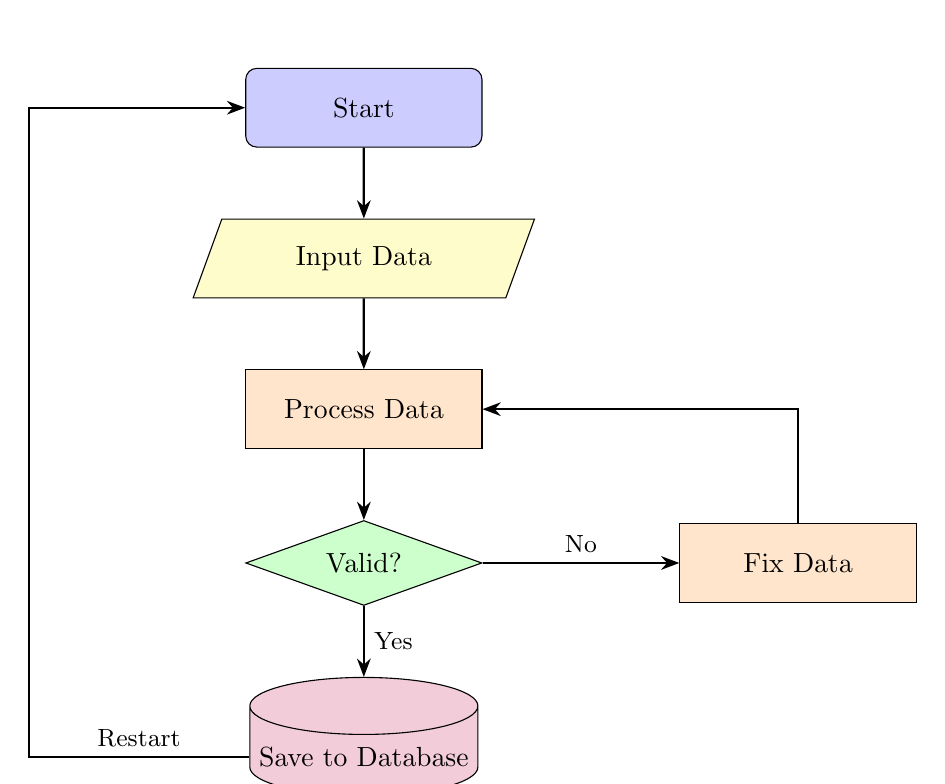
\begin{tikzpicture}[node distance=0.9cm and 2.5cm]
    % Nodes
    \node (start) [startstop] {Start};
    \node (in1)   [io,       below=of start] {Input Data};
    \node (pro1)  [process,  below=of in1]   {Process Data};
    \node (dec1)  [decision, below=of pro1]  {Valid?};
    \node (pro2)  [process,  right=of dec1]  {Fix Data};
    \node (db)    [database, below=of dec1]  {Save to Database};

    % Straight arrows
    \draw [arrow] (start) -- (in1);
    \draw [arrow] (in1)   -- (pro1);
    \draw [arrow] (pro1)  -- (dec1);

    % Labeled arrows
    \draw [arrow] (dec1) -- node[midway, right] {\small Yes} (db);
    \draw [arrow] (dec1) -- node[midway, above] {\small No}  (pro2);

    % Right-angled feedback loop
    \draw [arrow] (pro2.north) |- (pro1.east);

    % Restart arrow routed around the left side
    \draw [arrow] (db.west) -- ++(-2.8,0) node[midway, above] {\small Restart}
                  |- (start.west);
\end{tikzpicture}
\caption{TikZ flowchart with various shapes and arrow types.}
\label{fig:flowchart}
\end{figure}

\subsection{An Architecture Diagram}
The same toolkit works for system diagrams. \Cref{fig:arch} shows a typical web application, with the \texttt{fit} library drawing a dashed boundary around the backend.

\begin{figure}[htbp]
\centering
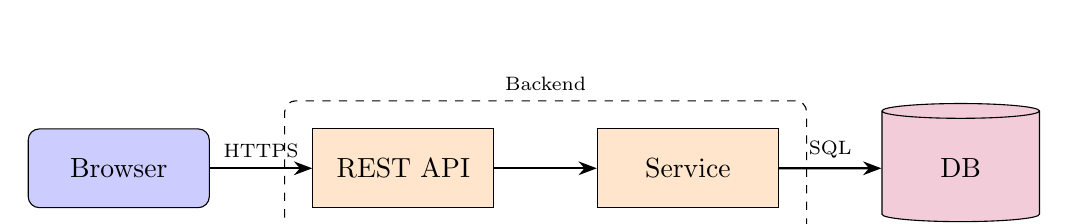
\begin{tikzpicture}[node distance=1.3cm,
    box/.style={process, minimum width=2.3cm}]
    \node (client) [startstop, minimum width=2.3cm] {Browser};
    \node (api)    [box, right=of client] {REST API};
    \node (svc)    [box, right=of api]    {Service};
    \node (db)     [database, right=of svc] {DB};

    \node [draw, dashed, rounded corners, fit=(api)(svc), inner sep=0.35cm,
           label={[font=\scriptsize]above:Backend}] {};

    \draw [arrow] (client) -- node[midway, above, font=\scriptsize] {HTTPS} (api);
    \draw [arrow] (api)    -- (svc);
    \draw [arrow] (svc)    -- node[midway, above, font=\scriptsize] {SQL} (db);
\end{tikzpicture}
\caption{A simple three-tier architecture drawn with TikZ.}
\label{fig:arch}
\end{figure}

% ============================================================
\section{Advanced Features: Code, Algorithms and Plots}
% ============================================================

\subsection{Displaying Code}
You can format source code beautifully using the \texttt{listings} package.
It supports syntax highlighting for over 80 programming languages.

\begin{lstlisting}[language=Python, caption={Python example with \texttt{listings}}]
def hello_world(name: str) -> None:
    """Greet someone by name."""
    print(f"Welcome to the Masterclass, {name}!")

# Call the function
hello_world("Abel")
\end{lstlisting}

\begin{lstlisting}[language=C, caption={C example}]
#include <stdio.h>

int main() {
    printf("Hello from C!\n");
    return 0;
}
\end{lstlisting}

\subsection{Typesetting Algorithms}
The \texttt{algorithm2e} package produces numbered pseudocode. \Cref{alg:bsearch} implements binary search.

\begin{algorithm}[htbp]
\caption{Binary search}\label{alg:bsearch}
\KwIn{Sorted array $A[1..n]$ and target value $t$}
\KwOut{Index of $t$ in $A$, or $-1$ if absent}
$lo \leftarrow 1$; \quad $hi \leftarrow n$\;
\While{$lo \le hi$}{
    $mid \leftarrow \lfloor (lo + hi)/2 \rfloor$\;
    \uIf{$A[mid] = t$}{
        \Return $mid$\;
    }
    \uElseIf{$A[mid] < t$}{
        $lo \leftarrow mid + 1$\;
    }
    \Else{
        $hi \leftarrow mid - 1$\;
    }
}
\Return $-1$\;
\end{algorithm}

\subsection{Plotting Data}
Using \texttt{pgfplots}, we can draw graphs natively---no Excel screenshots required!

\begin{figure}[htbp]
\centering
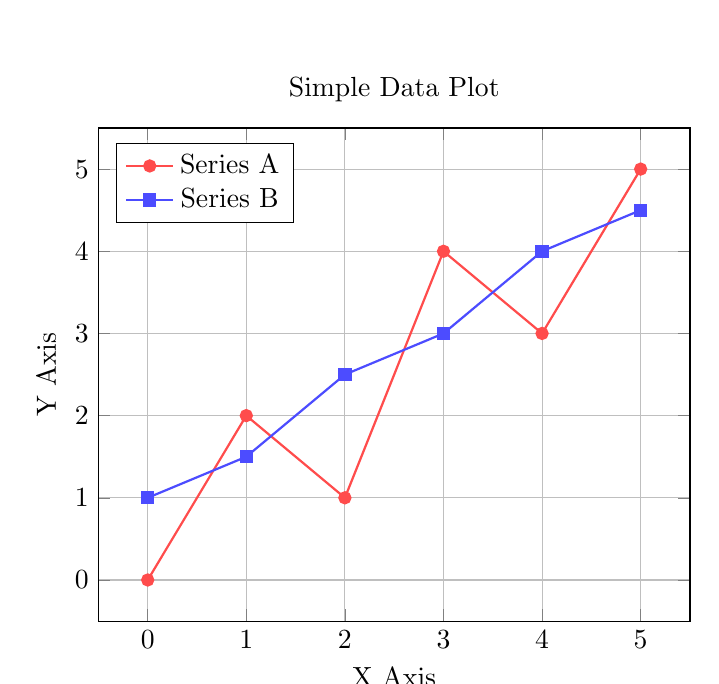
\begin{tikzpicture}
\begin{axis}[
    title={Simple Data Plot},
    xlabel={X Axis},
    ylabel={Y Axis},
    grid=major,
    width=0.75\textwidth,
    legend pos=north west
]
\addplot[color=red!70, mark=*, thick] coordinates {
    (0,0) (1,2) (2,1) (3,4) (4,3) (5,5)
};
\addplot[color=blue!70, mark=square*, thick] coordinates {
    (0,1) (1,1.5) (2,2.5) (3,3) (4,4) (5,4.5)
};
\legend{Series A, Series B}
\end{axis}
\end{tikzpicture}
\caption{A line graph with two series, generated natively in \LaTeX.}
\label{fig:plot}
\end{figure}

\subsection{Function Plots and Bar Charts Side by Side}
Plots can be generated from formulas or from data, and the \texttt{subcaption} package lays them out together (\cref{fig:sub}).

\begin{figure}[htbp]
\centering
\begin{subfigure}[t]{0.48\textwidth}
    \centering
    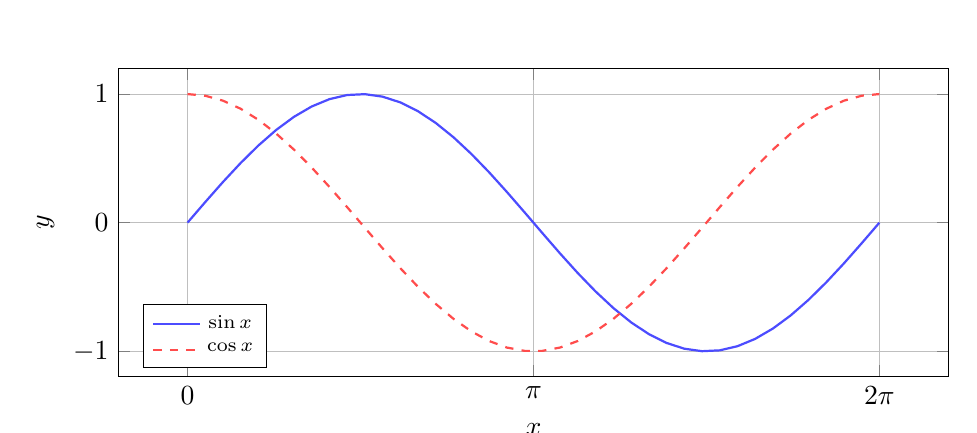
\begin{tikzpicture}
    \begin{axis}[width=\linewidth, height=5.5cm, xlabel={$x$}, ylabel={$y$},
                 grid=major, xtick={0,3.14159,6.28318},
                 xticklabels={$0$,$\pi$,$2\pi$}, legend pos=south west,
                 legend style={font=\scriptsize}]
    \addplot[domain=0:6.28318, samples=40, blue!70, thick] {sin(deg(x))};
    \addplot[domain=0:6.28318, samples=40, red!70, thick, dashed] {cos(deg(x))};
    \legend{$\sin x$, $\cos x$}
    \end{axis}
    \end{tikzpicture}
    \caption{Sine and cosine from formulas.}
\end{subfigure}
\hfill
\begin{subfigure}[t]{0.48\textwidth}
    \centering
    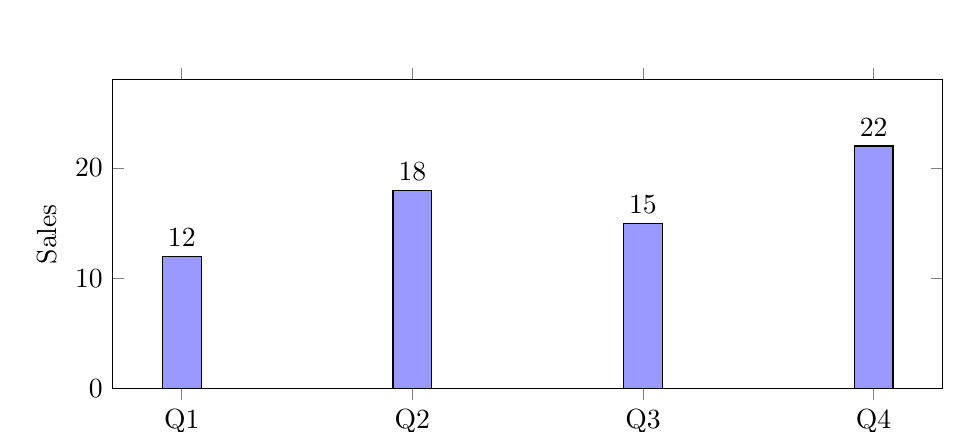
\begin{tikzpicture}
    \begin{axis}[ybar, width=\linewidth, height=5.5cm, symbolic x coords={Q1,Q2,Q3,Q4},
                 xtick=data, ymin=0, ymax=28, nodes near coords, bar width=14pt,
                 ylabel={Sales}]
    \addplot[fill=blue!40] coordinates {(Q1,12) (Q2,18) (Q3,15) (Q4,22)};
    \end{axis}
    \end{tikzpicture}
    \caption{Quarterly sales from data.}
\end{subfigure}
\caption{Two kinds of \texttt{pgfplots} charts in one figure.}
\label{fig:sub}
\end{figure}

\subsection{A 3D Surface}
\texttt{pgfplots} also draws surfaces. \Cref{fig:surface} shows the Gaussian $z = e^{-x^2-y^2}$.

\begin{figure}[htbp]
\centering
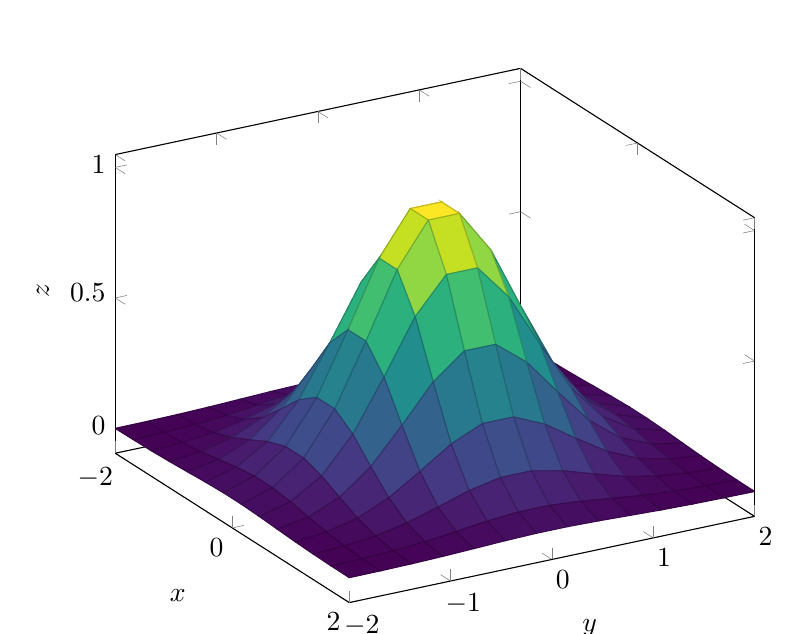
\begin{tikzpicture}
\begin{axis}[view={60}{30}, width=0.8\textwidth, xlabel={$x$}, ylabel={$y$},
             zlabel={$z$}, colormap/viridis]
\addplot3[surf, domain=-2:2, samples=14] {exp(-x^2-y^2)};
\end{axis}
\end{tikzpicture}
\caption{A 3D surface plot of a Gaussian.}
\label{fig:surface}
\end{figure}

% ============================================================
\section{Citations}
% ============================================================
Managing references is fully automatic. For example, we might want to cite a famous paper by Einstein~\cite{einstein1905}.
You just need to have the entry in your \texttt{references.bib} file and use \verb|\cite{key}|.
\LaTeX\ and BibTeX handle all the formatting and bibliography generation. Several keys can be cited together, such as the classic works on \LaTeX\ and literate programming~\cite{lamport1994, knuth1984, mittelbach2004}, or Shannon's founding paper on information theory~\cite{shannon1948}.

A minimal \texttt{references.bib} entry looks like this:
\begin{lstlisting}[language=TeX, caption={A BibTeX entry}]
@article{shannon1948,
  author  = {Shannon, Claude E.},
  title   = {A Mathematical Theory of Communication},
  journal = {Bell System Technical Journal},
  year    = {1948}
}
\end{lstlisting}

\begin{tipbox}
After adding a new citation, compile twice (Overleaf does this automatically). The first pass collects the keys and BibTeX builds the list. Later passes resolve the numbers.
\end{tipbox}

% ============================================================
\section{Overleaf Workflow Tips}
% ============================================================
\begin{enumerate}
    \item \term{Organize files.} Keep figures in \texttt{images/} and split long documents into files pulled in with \verb|\input|.
    \item \term{Use comments.} Anything after \texttt{\%} is ignored, which is useful for notes and for disabling code.
    \item \term{Read the log.} Fix the \emph{first} error, because later ones are often side effects.
    \item \term{Collaborate.} Share a link, track changes, and use the History feature to restore earlier versions.
    \item \term{Let AI help.} Describe the table, equation or diagram you want and paste the generated code, then check it compiles.
\end{enumerate}

% ============================================================
\section{Conclusion}
% ============================================================
This document touched on text formatting, lists, mathematics, theorems, tables, figures, diagrams, code, algorithms, plots and citations. Each feature is a small amount of text that \LaTeX\ turns into consistent, professional output. Try editing any example and recompiling to see the effect.

% --- BIBLIOGRAPHY ---
\bibliographystyle{plain}
\bibliography{references}

% ============================================================
\appendix
\section{Troubleshooting Common Errors}
% ============================================================
\begin{table}[htbp]
    \centering
    \caption{Frequent compile problems and fixes.}
    \label{tab:errors}
    \begin{tabularx}{\textwidth}{>{\raggedright\ttfamily\arraybackslash}p{4.6cm}X}
        \toprule
        \textbf{Message} & \textbf{Usual cause and fix} \\
        \midrule
        Undefined control sequence & A command is misspelled or its package is not loaded. \\
        File not found & Wrong path or capitalization of an image or \texttt{\textbackslash input} file. \\
        Missing \$ inserted & Math symbols such as \texttt{\_} or \texttt{\textasciicircum} used outside math mode. \\
        Citation undefined & Key missing from the \texttt{.bib} file, or not compiled twice yet. \\
        Overfull \textbackslash hbox & A line is too wide; rephrase or allow hyphenation. \\
        \bottomrule
    \end{tabularx}
\end{table}

\end{document}
